% Chapter 7

\chapter{The Parvovirus Life Cycle} % Main chapter title

\label{Chapter7} % For referencing the chapter elsewhere, use \ref{Chapter2} 

% \lhead{Chapter 2. \emph{Methods}} % This is for the header on each page - perhaps a shortened title

%----------------------------------------------------------------------------------------
\section{Receptor Binding}
\label{Binding}
Recognition of cell surface receptors by a virus enables the first step of infection and hence, represents a key parameter of tropism and pathogenesis (see chapter~\ref{Chapter5}, p.~\pageref{Chapter5}). Different biomolecules, as for instance proteins, carbohydrates, and glycolipids may serve as primary attachment factors. To date, a variety of different receptor molecules with specific binding properties or functional activities have been identified for some members of the subfamily~\textit{Parvovirinae} (See table~\ref{Tab: Receptors}, p.~\pageref{Tab: Receptors}. For a review see reference \cite{Receptor}). These include for example the AMDV-binding protein (ABP) for AMDV \cite{pmid10196278}, the globoside erythrocyte P antigen, in addition with $\alpha$\textsubscript{5}$\beta$\textsubscript{1}-integrin and Ku80 for B19V \cite{pmid8211117, pmid15661151, pmid12907437, pmid16076874, weigel}, transferrin receptors (TfRs) for CPV, FPV and MEV \cite{pmid16040076, pmid11264378} and heparan sulfate proteoglycan (HSPG), $\alpha$\textsubscript{\RM{5}}$\beta$\textsubscript{5}-integrin, and growth factor receptors for AAVs \cite{pmid14502277, pmid15596854, pmid9883842, pmid9445046, pmid9883843, pmid8599196}. However, recent studies conducted on B19V failed to verify an interaction of B19V with $\alpha$\textsubscript{5}$\beta$\textsubscript{1}-integrin. Instead, purified, recombinant VP1u was demonstrated to bind and internalize independently of the B19V capsid. VP1u binding and internalization was tightly restricted to few cell lines of the erythroid cell lineage only. These results, together with the ability of singly expressed VP1u to efficiently prevent B19V endocytosis, indicate that an unknown receptor with an expression pattern confined to few erythroid cell types mediates B19V internalization \cite{pmid24067971}.  

However, for most of the parvoviruses only the glycan component of their specific receptor is known. Glycans, which are carbohydrate polymers, represent the major components of the cell surface, thus providing a vast collection of important cellular attachment factors for viruses in general. They may be conjugated with cell surface proteins or membrane lipid head groups to form glycoproteins and glycolipids, respectively, or constitute glycosaminoglycan (GAG) chains attached to proteoglycans \cite{pmid16019714}. The extensive heterogeneity of the carbohydrate polymers which are expressed between different species, and even between different tissues within the same species, creates an immense variability in viral tissue tropism. This diversity is even further enlarged by various glycosidic linkage positions between each individual monosaccharide and by the high degree of chemical modifications of hydroxyl groups \cite{pmid11841250, pmid17632542}. Most commonly, sialic acids (SA) or sulfated oligosaccharide motifs of GAGs (e.g. heparan sulfate (HS)) form the distal, and therefore most surface exposed, units of glycoepitopes \cite{pmid17072005}.


Biochemical studies utilizing neuraminidase and proteinase K treatment have shown that SA is a common primary attachment factor for several parvoviruses infecting different species, as for example MVM \cite{pmid3296697, pmid16415031}, H1-PV \cite{pmid22258256}, BPV \cite{pmid15750863, pmid9747725, pmid15269359}, PPV \cite{pmid20484503}, AAV1 \cite{pmid16943302, pmid16940521}, AAV4, AAV 5 \cite{pmid15761263, pmid11435568, pmid11262413, pmid16409121}, CPV and FPV \cite{pmid1329321, pmid7975239}. However, SA-CPV and SA-FPV interactions are not sufficient for infectivity but require additional binding to their respective TfRs on canine and feline cells \cite{pmid1329321, pmid12525605, pmid11264378, pmid12885908}. More than 60 analogues of SA occur in nature which result from modifications to the nine-carbon backbone \cite{pmid17072005} and are estimated to be present at 5~$\times$~10\textsuperscript{5} copies per cell on A9 mouse fibroblasts \cite{pmid20517, pmid6602221}. The SA binding pocket of MVM was identified by analysis of SA soaked into preformed crystals of virus-like particles (VLPs)\footnotemark of MVMp. Structurally, the SA electron density is associated with the dimple-like depression located at the icosahedral two-fold axis in the MVM cpasid (see figure~\ref{Morphology}, p.~\pageref{Morphology}). The binding pocket exposes highly positive charges which interact with SA moieties on the cell surface \cite{pmid16415031}. Interestingly, the localization of the SA binding domain in MVM is proximal to the CPV and FPV determinants of SA binding to erythrocytes \cite{pmid7645206, pmid8392729, pmid1329321, pmid10884355}. Significantly, the amino acids determining \textit{in vitro} tropism (317 and 321) and \textit{in vivo} pathogenicity (325, 362, and 368) for MVM invariably localize in close vicinity of the SA binding pocket (see chapter~\ref{Chapter5}, p.~\pageref{Chapter5}) \cite{pmid16103145}.                  

The identification of virus receptors and the characterization of virus-receptor interactions are of great relevance for understanding virus evolution, host tropism, and pathogenesis. A profound knowledge of the first steps of viral infections on the host cell surface is indispensable for the development of antiviral therapies and for the construction of gene therapy vectors with determined targeting.    


\footnotetext{VLPs are non-infectious particles which do not contain any viral genetic material. The expression of parvoviral structural proteins results in a spontaneous self-assembly of VLPs. Since VLPs mimic the organization and conformation of viral surface epitopes, they can elicit strong B cell and T cell immune responses. Therefore, they provide a useful tool for the development of vaccines.}

\begin{small}
\begin{center}

\begin{longtable}{P{0.7in} P{1.65in} P{1.45in} P{0.6in} P{0.8in}}
\caption[Parvoviruses and their receptors]{\normalsize Parvoviruses and their receptors}\\
\\
\label{Tab: Receptors}
\normalsize\textbf{Virus} & \normalsize\textbf{Receptor} & \normalsize\textbf{Coreceptor} & \normalsize\textbf{Host} & \normalsize\textbf{Reference}\\
\hline
\endfirsthead % all the lines above this will be repeated on every page

\multicolumn{3}{l}{\normalsize\textbf{Table~\ref{Tab: Receptors}} continued}\\
\\
\normalsize\textbf{Virus} & \normalsize\textbf{Receptor} & \normalsize\textbf{Coreceptor} & \normalsize\textbf{Host} & \normalsize\textbf{Reference}\\
\hline
\endhead

\hline
\multicolumn{5}{l}{This table was adapted from reference \cite{Halder}}
\endlastfoot

AAV1 & $\alpha$2-3 and $\alpha$2-6 N-linked sialic acid & - & Human & \cite{pmid16940521} \\
AAV2 & HSPG & Integrin $\alpha$\textsubscript{5}$\beta$\textsubscript{1}, $\alpha$\textsubscript{\RM{5}}$\beta$\textsubscript{5}, FGFR1, HGFR, LamR & Human & \cite{pmid16973587, pmid15596854, pmid9883842, pmid9883843, pmid9445046, pmid16940508} \\
AAV3 & HSPG & HGFR, LamR, FGFR1 & Human & \cite{pmid16973587, pmid20545554, pmid16195782} \\
AAV4 & $\alpha$2-3 O-linked sialic acid & - & NHP & \cite{pmid11435568} \\
AAV5 & $\alpha$2-3 and $\alpha$2-6 N-linked sialic acid & PDGFR & Human & \cite{pmid14502277, pmid16409121, pmid11262413, pmid11435568} \\   
AAV6 & $\alpha$2-3 and $\alpha$2-6 N-linked sialic acid, HSPG & EGFR, & Human & \cite{pmid20473307, pmid16940521, pmid16943302} \\  
AAV8 & - & LamR & NHP & \cite{pmid16973587} \\
AAV9 & Galactose & LamR & Human & \cite{pmid16973587, pmid21576824, pmid21330365} \\
Bovine AAV & Gangliosides, chitotriose & - & Bovine & \cite{pmid20231878, pmid16699032} \\
AMDV & AMDV-binding protein (ABP) & - & Mink & \cite{pmid10196278} \\
BPV1 & Sialic acid & Glycophorin A & Bovine & \cite{pmid15750863, pmid9747725} \\
B19V & Erythrocyte P antigen & Integrin $\alpha$\textsubscript{5}$\beta$\textsubscript{1}, ku80 & Human & \cite{pmid8211117, pmid15661151, pmid12907437, pmid16076874, weigel} \\
MVM & Sialic acid & - & Rodent & \cite{pmid3296697, pmid15229399, pmid16822863} \\
CPV/FPV & Sialic acid & Transferrin receptor & Cat, dog & \cite{pmid11264378, pmid12525605} \\
PPV & Sialic acid & - & Swine & \cite{pmid20484503} \\

     
\end{longtable}
\end{center} 
\end{small}


\section{Receptor-mediated Endocytosis}
\label{Endocytosis}
All known parvoviruses enter the host cell by receptor-mediated endocytosis, using a wide variety of partially unknown glycosylated receptor molecules, exposed on the cell surface \cite{pmid18406140} (see table~\ref{Tab: Receptors}, p.~\pageref{Tab: Receptors}). The endocytic route offers two important advantages for karyophilic viruses. On the one hand, the capsids are transported rapidly and efficiently towards the nuclear periphery. On the other hand, the exposure to low pH enables the capsid to undergo conformational changes which are required for further stages of infection (see section~\ref{Rearrangements}, p.~\pageref{Rearrangements}), such as endosomal escape, uncoating, and nuclear localization. Latest research demonstrated that, in addition to the classical clathrin-mediated endocytosis (CME) \cite{pmid20484503, pmid10559355, pmid10644365}, several alternative endocytic routes can be used by parvoviruses. For example, AAV2 utilizes clathrin-independent carriers (CLICs) \cite{pmid22177561}, AAV5 uses caveolae-dependent endocytosis \cite{pmid19141440}, and PPV utilizes macropinocytosis \cite{pmid20484503} as additional endocytic pathways. Most recently, Garcin and Panté showed that MVM enters its host cell by at least three potential endocytic routes. Inhibition of various endocytic pathways with specific drugs in combination with electron microscopy (EM), immunofluorescence microscopy (IF), and fluorescence-activated cell sorting (FACS), identified clathrin-, caveolin-, and CLIC-mediated endocytosis for MVM. However, the latter endocytic uptake mechanism was restricted to transformed cells only, but did not occur in murine A9 fibroblasts. This observation was confirmed in additional experiments which demonstrated that dynasore, an inhibitor of dynamins, completely blocked MVMp uptake in A9 mouse fibroblasts, whereas its inhibitory effect was incomplete in transformed cells. These results indicate that both clathrin- and caveolin-mediated MVMp endocytosis is dependent on dynamin in murine A9 fibroblasts, but transformed cells allow for the dynamin-independent CLIC-mediated uptake of MVMp \cite{pmid25863880}. Although parvoviruses share some general features in receptor binding and in their routes of cellular entry, each appears to evince its own mechanistic details that do not allow for generalization.     

\section{Endosomal Trafficking and Capsid Rearrangements}
\label{Rearrangements}
Endosomal trafficking of parvovirus virions is reported to be a slow and rate-limiting process in viral infection \cite{pmid10841516, pmid10623762, pmid11287557, pmid16379002}. The delayed progression to infection allows parvoviruses to undergo important structural transitions and prolonged processing within endosomes. AAVs for instance escape from early endosomes, but reach the nucleus only after 40 min to 2 hours post-infection (hpI) \cite{pmid10684294, pmid12388712}. MVM belongs to the best characterized parvoviruses with respect to endosomal trafficking in spite of the rapid dynamics and complexity of viral movement within and between endosomal compartments. It is reported to traffic even slower through the endocytic pathway and reaches the cell nucleus only after 8 hpI when DNA replication was detected \cite{pmid12438589}.       

Several lines of evidence confirm that endosomal processing of incoming parvovirus particles is essential. Next, virions with or without exposed N-VP2 termini failed to confer a nuclear localization phenotype to AAV2 when directly injected into the cytoplasm to bypass the endocytic pathway \cite{pmid16956943, pmid15829993}. Similarly, low pH pre-treated CPV capsids were unable to accumulate in the nucleus following injection into the cytoplasm \cite{pmid9420290}. Last, for MVM, all structural rearrangements were equally impaired by lysosomotropic drugs, thereby preventing infection \cite{pmid16379002, pmid12438589}. These drugs, such as bafilomycin A\textsubscript{1} or the weak base chloroquine diphosphate, raise the endosomal pH by inhibiting the vacuolar-type H\textsuperscript{+}-ATPase \cite{pmid2973058, pmid6094416, BafA1} or by accumulation inside acidic compartments \cite{pmid4606365, pmid28524, pmid6169733}, respectively. Finally, endosomal acidification has been demonstrated to be essential for the infection of AAV \cite{pmid10684294, pmid15681453, pmid11160681, pmid11287557}, CPV \cite{pmid10644365, pmid9420290, pmid1733094}, and MVM \cite{pmid16379002, pmid12438589}.  

Three considerable structural rearrangements of the MVM capsid were observed to occur simultaneously, starting 30 min after endocytosis. The capsid transitions include the cleavage of the exposed N-VP2 termini, the externalization of originally sequestered N-VP1 termini, and the release of the full-length viral DNA genome without loss of capsid integrity \cite{pmid16379002}. The conformational changes of parvovirus capsids which are induced by endosomal trafficking \textit{in vivo}, partially can be mimicked \textit{in vitro}. Treatment of CPV particles under acidic conditions that mimic endosomal pH induced VP1u exposure \cite{pmid14644609}. However, in the case of MVM full capsids (FC), prior cleavage of N-VP2 termini to VP3 is a prerequisite for VP1u externalization under such conditions \cite{pmid9927584, pmid16352540}. Contrarily, the N-VP2 termini remained buried in the interior of empty capsids (EC) and thus they were not accessible to proteolytic digestion \cite{pmid16379002}. Surprisingly, EC exposed the N-VP1 termini with similar kinetics to FC, indicating that at least for EC, neither the genomic DNA nor the cleavage of N-VP2 is involved in the extrusion of N-VP1 \cite{pmid9927584, pmid16379002}. Harsh conditions, such as exposure to heat or urea, trigger VP1u externalization in AAV \cite{pmid15827144}, CPV \cite{pmid11799183, pmid9770425}, and MVM particles \cite{pmid9927584, pmid19955311}. Although artificial \textit{in vitro} treatments can not directly reproduce the \textit{in vivo} stimuli they enabled the biochemical and structural characterization of capsid dynamics \cite{pmid9927584, pmid19955311, pmid15827144, pmid11799183}. The differences observed in the \textit{in vitro} and \textit{in vivo} studies imply that a combination of several factors, such as receptor binding, low endosomal pH, or interactions with unknown host factors play a role in these structural transitions of parvoviruses.       

The fact that the bulk of incoming particles are retained within lysosomal compartments, and only a small proportion escapes the endocytic route (see section~\ref{Escape}, p.~\pageref{Escape}), impedes the study of the infectious pathway of parvoviruses. Moreover, the lack of dynamic information in fixed cell samples complicated the study of virus trafficking through the highly dynamic and overlapping vesicular endocytic pathway. However, emerging advances in time-lapse microscopy make live cell imaging an important method to shed light into the complex nature of endosomal trafficking in future.





 

\section{Endosomal Escape}
\label{Escape}
The high particle to infection (P/I) ratio\footnotemark of most parvoviruses (100:1 to >1000:1) \cite{pmid4673484, pmid20649475, pmid7288919} indicates that most of the incoming viruses fail to navigate the nucleus. Indeed, a substantial portion of the incoming MVM virions was demonstrated to follow a non-infectious pathway ending up in lysosomal compartments where they co-localized with co-endocytosed dextrans which had a MW of 10 kDa and were used as lysosomal marker. Hence, the endosomal escape represents the major barrier for the subsequent steps of MVM infection. However, the inability to escape from the endocytic route was not due to a failure in endosomal processing of MVM since virions retained in lysosomal compartments underwent all required structural transitions. MVM VLPs or ECs that accumulated in lysosomes remained intact up to 50 hpI but the exposed, capsid-tethered viral DNA of FCs was degraded 21 hpI, most probably by the lysosomal endonuclease DNase~\RM{2} activity \cite{pmid16379002}. \footnotetext{The P/I ratio is the number of virus particles per plaque-forming unit (PFU).}

Non-enveloped viruses are, by their very nature, unable to deliver their genomes into the host cell by fusion with the cellular plasma or endosomal membrane, as achieved by enveloped viruses \cite{pmid18596815}. In order to breach their host cell's delimiting membrane they must employ alternative strategies. Although MVM was not yet directly demonstrated to permeabilize endosomal membranes, there is evidence that parvoviruses have the capability to disrupt membranes. Labeled dextrans with a MW of 3 kDa were progressively liberated into the cytosol 8-20 h after co-endocytosis with CPV virions. However, despite the apparent change in the permeability of endosomal membranes, there is no complete disintegration of endosomal vesicles since larger dextrans with a MW of 10 kDa, as well as $\alpha$-sarcin, were mainly retained in vesicles at the same time post-infection \cite{pmid14644609, pmid10644365}.

Several arguments speak in favor of the N-VP1 terminal PLA\textsubscript{2} activity (see section~\ref{PLA2}, p.~\pageref{PLA2}) mediating endosomal escape of parvoviruses. Firstly, N-VP1 becomes exposed in early endocytic vesicles \cite{pmid16379002, pmid14644609, pmid9927584, pmid16284249, pmid11961250, pmid20974479, pmid11702787}. Secondly, VP1 has been demonstrated to be essential for productive infection of parvoviruses in a step prior to the initiation of DNA replication \cite{pmid8416366, pmid10684294, pmid1733094, pmid11160681, pmid11287557, pmid10644365, pmid12438589, pmid9420290}. And thirdly, pre-incubation of N-VP1-exposing CPV virions with PLA\textsubscript{2} inhibitors, such as quinacrine and manoalide, significantly reduced or completely abolished infectivity, respectively \cite{pmid14644609}. For MVM \cite{pmid16284249} and AAV2 \cite{pmid20974479}, complementation assays between wild-type and mutant particles have been used to demonstrate that the lipolytic PLA\textsubscript{2} function is mediating phospholipid bilayer penetration. Therefore, mutants with amino acid substitutions within their catalytic dyad (see section~\ref{PLA2}, p.~\pageref{PLA2}) were constructed. Their enzymatic activity was severely impaired and viral infectivity was completely abrogated. Polyethyleneimine-induced endosomal rupture or co-infection with wild-type or mutant virions could partially rescue the mutant phenotype. Similarly, co-infection with endosomolytically active adenoviral variants resulted in a partial complementation of the mutant phenotype. Contrarily, endosomolytically inactive adenoviral variants, as well as wild-type ECs carrying sequestered VP1u sequences, were unable to restore infectivity of the PLA\textsubscript{2}-negative mutants. Thus, the capsid-tethered PLA\textsubscript{2} motif seems to be either directly or indirectly required for successful penetration of the endosomal membranes.  

Information about the site of endosomal escape for MVM is still lacking. Previous \textit{in vitro} experiments showed that the optimal pH for the parvoviral PLA\textsubscript{2} enzymatic activity ranges between pH 6 to 7, but drastically decreases at a pH below 5 \cite{pmid14726513}. Correspondingly, the acidic, lysosomal environment would not provide optimal conditions for PLA\textsubscript{2}-mediated escape from the degradative pathway. Therefore, it is tempting to speculate that only a few viruses manage to escape the endocytic route from a pre-lysosomal compartment in the absence of vesicle disintegration. This hypothesis is supported by the fact that MVM externalizes N-VP1 already within the first minutes of infection, thus exposing the functional PLA\textsubscript{2} enzymatic activity on its surface. Additionally, brefeldin A, a fungal antibiotic that blocks the transition between early and late endosomes \cite{pmid1682055}, has been demonstrated to abrogate MVM infection \cite{pmid12438589}. In summary, these results suggest that the minority of virions that enter the cytosol escape from an intermediate pre-lysosomal vesicle, namely late endosomes \cite{pmid16379002}.

%Endosomal escape might be heavily restricted because the endocytic route is highly dynamic, showing significant differences in pH, and virions must undergo all required structural transitions within a tight time frame. Accordingly, successful escape only occurs if both requirements are fully accomplished.      

    






\section{Cytosolic Trafficking and Interactions with the Proteasome}

\section{Nuclear Targeting}
\label{Localization}      
Apart from the plasma membrane, the nuclear envelope constitutes a second barrier to karyophilic viruses. They need to enter the host's nucleus in order to profit from the replication and transcription machinery for their own multiplication. In fact, viral structural components enter the nucleus at two stages of their life cycle. Initially, when the incoming virion delivers its genome and late in infection, when viral subunits accumulate in the nucleus for self-assembly leading to the generation of virus progeny. Small molecules freely diffuse through the nuclear pore complex (NPC). In contrast, nuclear import of larger macromolecules, between 9 and 39 nm in diameter \cite{pmid11854401}, is highly selective and depends on energy and temperature. The nuclear translocation across the NPC is mediated through import signals exposed on the cargo molecules in conjunction with soluble transport receptors \cite{pmid14570049, pmid14504656, pmid15702987}. 

\subsection{Nuclear translocation of the incoming virion}
Interestingly, the diameter of the NPC central channel \cite{pmid11854401, pmid2450095} is in the range of the 25 nm diameter of the parvovirus capsid \cite{NPC}. Therefore, incoming parvoviruses could physically traverse the NPC fully intact without partial or complete capsid uncoating, as it has been reported for more complex viruses, such as influenza- or retrovirusus \cite{pmid10848617, pmid11389849, pmid8970960, pmid11031249, pmid9891810}. In the absence of nuclear membrane disintegration, the transport of viral particles must proceed across the NPC \cite{pmid10801463, pmid10395558, pmid11448991}, as it is the case for cellular proteins. However, there is evidence that MVM enters the host's nuclei in a NPC-independent way \cite{pmid17030854}. When microinjected into the cytoplasm of \textit{Xenopus oocytes}, MVM has been demonstrated to cause damage to the nuclear envelope in a time- and concentration-dependent manner \cite{pmid16298969}. It is supposed that MVM hijacks a cellular mechanism to disrupt the nuclear envelope. MVM-mediated, non-apoptotic caspase-3 activity induces nuclear entry of MVM capsids and possibly further accessory proteins required for replication. The detailed mechanism remains elusive but involves the re-localization of caspase-3 from the cytoplasm to the nucleus without its activation above basal levels in MVM infected cells. In the nucleus, the protease was demonstrated to cleave lamin B2, resulting in a sustained disruption of the nuclear lamina structure and progression of nuclear envelope rupture. Inhibition of caspase-3 during MVM infection resulted in a significant reduction of nuclear entry of MVM capsids and delayed expression of early viral gene products. These results support the aforementioned mechanism of a caspase-facilitated disruption of the nuclear envelope \cite{pmid21367902}.  


Several observations are in line with a nuclear translocation of MVM as entirely intact particle. Even though the NLM domain (see section~\ref{NLM1}, p.~\pageref{NLM1}) is disposed at the inner surface of the capsid \cite{pmid9817841}, the structural rearrangements of MVM during the early endosomal trafficking (see section~\ref{Rearrangements}, p.~\pageref{Rearrangements}) allow the externalization of the VP1u sequence. In this way, the basic NLS sequences (see section~\ref{NLS1}, p.~\pageref{NLS1}) become exposed on the capsid surface. The exposed BC sequences might direct the incoming particle towards the nucleus. Accordingly, deletions of BC1 to BC4 sequences within VP1u completely abrogated MVM infectivity \cite{pmid12072505}. Similarly, cytoplasmic microinjection of VP1u-specific antibodies was able to neutralize CPV infection \cite{pmid11799183}. However, nuclear translocation of MVM as a stable disassembly intermediate remains possible since the generation of BC1-4 mutant virions required nuclear localization competent, NLM-harboring viral protein subunits. Hence, although MVM particles composed of only VP2 subunits are insufficient for MVM infection \cite{pmid8416366}, the NLM in the common part of VP1 and VP2 might cooperatively participate together with the BC sequences in the process of nuclear localization \cite{pmid12072505}.

Currently, it is still controversial whether parvoviruses enter the nucleus as whole particles or as partial disassembly intermediates. CPV particles microinjected into the cytoplasm slowly entered the nucleus possibly across the NPC and were detectable by antibodies against intact capsids, indicating that nuclear entry occurs without extensive uncoating \cite{pmid12970411, pmid10775624}. Other reports describe alternative, NPC-independent nuclear import mechanisms for intact AAV particles when co-infected with adenoviruses \cite{pmid11592830, pmid12388712}. However, nuclear translocation of intact AAV particles was inefficient \cite{pmid16140755, pmid10684294, pmid11729319} or even not detectable \cite{pmid16956943} in the absence of the helper virus, suggesting viral uncoating before or during nuclear entry.

\subsection{Nuclear translocation of the structural proteins}
\label{Struc Transloc}
The structural proteins of MVM translocate to the nucleus using different mechanisms although sharing a common C-terminal sequence with VP1 extending along additional 142 amino acids at its N-terminus. Deletions in any part of the VP2 sequence prevented the major viral protein from nuclear import, indicating that nuclear translocation is mediated by a conformational NLM (see section~\ref{NLM1}, p.~\pageref{NLM1}) requiring the correct cytoplasmic folding of the whole polypeptide. In contrast, VP1 was not retained in the cytoplasm in spite of harboring the same deletions within the common amino acid sequence to VP2 \cite{pmid10729155}. VP1 is actively imported by clusters of basic amino acids, referred to as NLS (see section~\ref{NLS1}, p.~\pageref{NLS1}), within its VP1u region \cite{pmid12072505}. These basic clusters show high homology to conventional NLS of many karyophilic polypeptides (see figure~\ref{NLS}, p.~\pageref{NLS}) \cite{pmid2004116, pmid6088992}. 

Lombardo \textit{et al.} demonstrated that VP1 was able to cooperatively interact with NLM incompetent VP2 subunits, resulting in a predominant accumulation of VP2 in the nucleus in around 40~\% of the transfected cells. Such coupling of capsid proteins and cooperative nuclear import has also been shown for AAV2 \cite{pmid1331503}. The efficient nuclear import of NLM-deficient VP2 is surprising since MVM VP1 and VP2 subunits are expressed in a 1:5 stoichiometry. Correspondingly, there is evidence that each VP1 subunit interacts with two VP2 subunits to form a trimer which represents the stable precursor in the MVM assembly pathway \cite{pmid10729155}. Large insertion loops between the $\beta$G and $\beta$H strands (see figure~\ref{Structure1}, p.~\pageref{Structure1}) of threefold symmetry-related subunits extensively interact with each other \cite{pmid8377200, pmid8969301} to form the threefold spikes of parvoviral virions \cite{pmid9817841, pmid2006420}. This observation reinforces the hypothesis of a stable VP trimer as assembly precursor \cite{pmid10729155}. Indeed, covalent crosslinking of assembly intermediates revealed two types of oligomeric assembly units. The larger species, a heterotrimer, contains one VP1 and two VP2 subunits whereas the smaller homotrimer consist of only VP2 subunits \cite{pmid16469332}. Moreover, the stable trimeric assembly intermediates have been directly demonstrated by the use of atomic force microscopy (AFM) \cite{pmid22713577}.     

The NLS and NLM, which represent functional nuclear import sequences of MVM, may be involved as major regulatory elements at several levels of MVM morphogenesis. Firstly, they maintain the stoichiometry between the viral protein subunits in the host's nuclei. Secondly, nuclear translocation capacity is only conferred to a specific subviral assembly intermediate, namely the VP trimer, thus organizing capsid assembly in the nucleus. Thirdly, correct folding of the polypeptide chains is a prerequisite for efficient nuclear translocation. Misfolded proteins are excluded from nuclear entry, hence preventing from detrimental interference with MVM capsid assembly in the nuclei \cite{pmid10729155}.

Nuclear translocation of the viral structural proteins depends on the cell cycle. In human and mouse fibroblasts synchronized at G\textsubscript{0}, G\textsubscript{1}, and G\textsubscript{1}/S transition, VPs accumulated in the cytoplasm. Upon arrest release, VPs translocated to the nucleus contemporaneously when the cell entered S phase. In the nucleus they immediately assembled into capsids (see section~\ref{Assembly}, p.~\pageref{Assembly}) \cite{pmid26067441}.                

 
\nomenclature{AFM}{Atomic force microscopy}


\section{NS2}
NS2 was demonstrated to have a critical role in MVM replication depending on the infected cell type. Following infection or transfection of restrictive murine cells with NS2-null mutants, little amount of mutant dsDNA replicative from (RF), and no detectable accumulation of progeny unit-length ssDNA genomes was detectable. However, the restricted replication of MVM genomes was less evident in permissive human cells \cite{pmid2147041}. Contrarily, NS2-Crm1-mutants produced dsDNA dRF and mRF levels comparable to those of the wild type at both early and late times post-transfection. Interestingly, the amount of accumulated viral progeny ssDNA drastically decreased in restrictive murine cells at proceeding times post-transfection. This observation suggests that the interaction of NS2 with Crm1 is dispensable for MVM dsDNA replication. However, it is strictly required for the production of progeny ssDNA, particularly in restrictive murine cells \cite{pmid11884550}.  




\section{Replication}
\label{Replication}
Due to the small capsid size of an approximate maximum external radius of 140 \r{A} \cite{pmid15299974}, the coding capacity of MVM genomic DNA is strictly limited. Consequently, the viral genes do not code for one's own DNA- and RNA polymerases and relevant accessory proteins. In order to efficiently initiate replication, MVM must recruit and assemble crucial cellular factors at one of its active origins of replication. Thus, viral proliferation heavily depends on ancillary cellular factors that are essentially involved in viral genome replication and transcription. These factors are transiently supplied by proliferating host cells during the S-phase in the nucleus \cite{pmid16789120, pmid6602221, pmid3005655, pmid3296697, pmid9418888, pmid4673484, S-phase}. In contrast to other small, host cell depending DNA viruses, as for instance SV40 \cite{pmid4291013, pmid16578647}, MVM does not have the capability to stimulate resting cells and to initiate its DNA replication. Infection of resting host cells results in an initial latent period until infected cells enter S-phase of their own volition in order to amplify its DNA \cite{pmid4673484, pmid3346950, pmid10792046}. For these reasons, MVM, and parvoviruses in general, show a pronounced predilection for rapidly dividing cell populations. 

Parvoviruses are unique among all known viruses in having a DNA genome that is both linear and single-stranded. Thus, it is not surprising that they evolutionary adapted their own one of a kind replication strategy. Their singular method to amplify the ssDNA genome resembles an ancient mechanism, known as rolling circle replication (RCR), that is utilized by many other small, circular prokaryotic and viral replicons \cite{pmid1630899, pmid8374079, pmid8824773, pmid9092519, pmid9010307}. However, in parvoviruses the RCR mechanism is modified and adapted for the replication of a linear chromosome. The parvoviral replication strategy, termed rolling hairpin replication (RHR), proceeds by a single-strand displacement mechanism, so there is no lagging-strand synthesis, and the integrity of the terminal hairpin sequences is maintained \cite{pmid967244}. The unidirectional progression of the replication fork results in the synthesis of a single, continuous DNA strand. In addition, MVM replication forks are aphidicolin-sensitive and require the proliferating cell nuclear antigen (PCNA). Such DNA elongation mechanism argues for a DNA synthesis that is mediated by DNA polymerase $\delta$ and its accessory proteins \cite{pmid10792046, pmid12050365, pmid9525597}. Initiation of parvovirus replication provokes the reorganization of the host cell nucleus, leading to formation of distinct nuclear foci, referred to as "autonomous parvovirus-associated replication" (APAR) bodies \cite{pmid11287588, pmid10775619, pmid11907229}. These bodies were shown to be active sites of viral replication and to accumulate essential cellular replication proteins such as cyclin A, DNA polymerases $\alpha$ and $\delta$, PCNA, and replication protein A (RPA) \cite{pmid10792046}. 

In the initial stage of the RHR, complementary strand synthesis starts from the left-end snap-back telomere, which serves as a primer for the generation of double-stranded monomeric replicative form (mRF) DNA (see step (i) in figure~\ref{RHR}, p.~\pageref{RHR}). Subsequently, the growing complementary strand is ligated to the flipped-back right-end telomere by a host ligase, resulting in a covalently continuous RF (cRF) species (see step (ii) in figure~\ref{RHR}, p.~\pageref{RHR}) \cite{pmid2911112, pmid2543770}. This monomer-length turnaround intermediate functions as a transcription template for NS1 expression. NS1 is essential for all further stages of the RHR pathway because the cellular replication machinery is unable to melt, copy, and re-orient the left-end telomere \cite{pmid8995615}. In the first instance, NS1 nicks the right-end telomere (\textit{OriR}) of the cRF intermediate \cite{pmid9349487}, assisted by a host DNA-bending protein from the high-mobility group 1/2 (HMG 1/2) family (see step (iii) in figure~\ref{RHR}, p.~\pageref{RHR}) \cite{pmid9765384}. The resulting, liberated, 3' nucleotide at the nick site serves as a platform for the assembly of a new replication fork. NS1 remains covalently attached to the 5' end of the mRF DNA, where it functions as the 3' to 5' replicative helicase \cite{pmid12050365, pmid3339715, pmid3203742}. The next step (see step (iv) in figure~\ref{RHR}, p.~\pageref{RHR}), called "hairpin transfer", involves reopening and copying of the right-end hairpin sequence in order to generate a right-end extended duplex molecule, replacing the original sequence of the right-end telomere (R) with its inverted complement (r). The two previous steps (iii and iv) of the RHR are commonly referred to as "terminal resolution" \cite{telomere2}. In a NS1 dependent reaction, the extended duplex RF is melted and refolded into two hairpins, creating a "rabbit-ear" structure (see step (v) in figure~\ref{RHR}, p.~\pageref{RHR}) \cite{pmid14997524, pmid12075084}. In this way, the path of the replication fork is reversed effectively, redirecting it back along the internal coding sequences (see step (vi) in figure~\ref{RHR}, p.~\pageref{RHR}). Finally, this results in the generation of dimeric RF (dRF) and higher-order concatemeric molecules (see steps (vii-ix) in figure~\ref{RHR}, p.~\pageref{RHR}), in such a way that the viral coding sequence is replicated twice as frequently as the telomeres. Viral genomes are fused through a single palindromic junction, in either a left-end:left-end or right-end:right-end orientation. In a last step, individual, unit-length, ssDNA genomes are excised and displaced from the concatemeric RF intermediates. Initially, they feed back as new templates into the replicative pool to promote exponential DNA amplification but later they are consumed by encapsidation \cite{pmid15681430, encapsidation}.     

\cite{pmid967244, pmid3973977, pmid3296697, pmid8995615}         


\begin{figure}[t]
\centering
  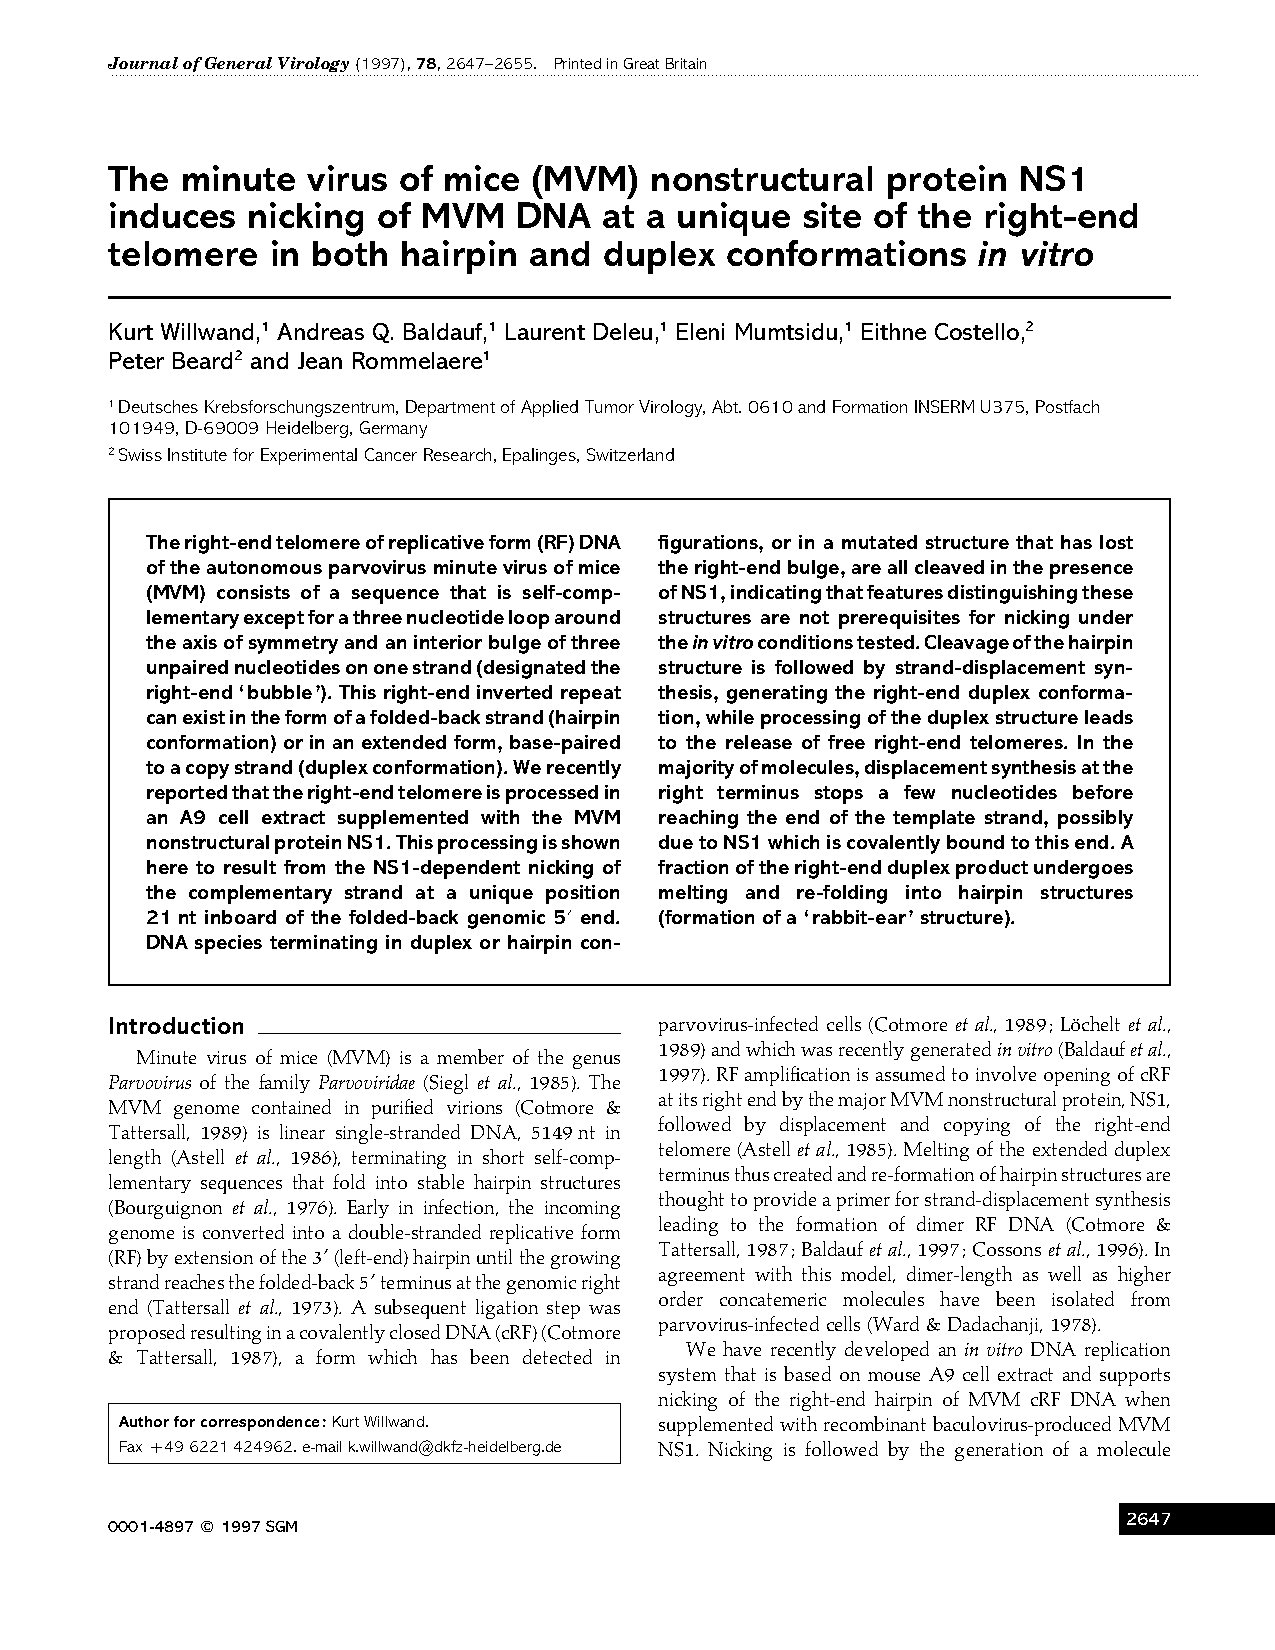
\includegraphics[scale=0.7]{Replication}
  \caption[Rolling hairpin replication (RHR)]
   {Modified rolling hairpin model for MVM DNA replication. The sequence of the parvoviral genome is illustrated by a continuous line, colored blue for the parental genome, yellow for progeny genomes, and black for newly synthesized DNA, the 3’ end of which is capped by an arrowhead. The green sphere represents NS1, which nicks the covalently closed monomer (cRF) and remains attached to its 5’ end. The letters L and R depict the palindromic sequences at each terminus, with their inverted complements represented by l and r, respectively. Red dashed boxes depict the turnaround (tr) form of the right-end and the dimer junction (dJ) form of the left-end palindrome \cite{els}. 
} 
\label{RHR}
\end{figure}

\nomenclature{RCR}{Rolling circle replication}
\nomenclature{RHR}{Rolling hairpin replication}
\nomenclature{mRF}{Monomeric replicative form DNA}
\nomenclature{cRF}{Closed replicative form DNA}
\nomenclature{dRF}{Dimeric replicative form DNA}
\nomenclature{HMG 1/2}{High mobility group proteins 1 and 2}
\nomenclature{PCNA}{Proliferating cell nuclear antigen}
\nomenclature{RPA}{Replication protein A}
\nomenclature{APAR}{Autonomous parvovirus-associated replication}
\nomenclature{HSPG}{Heparan sulphate proteoglycan}
\nomenclature{GAG}{Glycosaminoglycan}
\nomenclature{SA}{Sialic acid}
\nomenclature{HS}{Heparan sulfate}
\nomenclature{VLP}{Virus-like particle}
\nomenclature{CME}{Clathrin-mediated endocytosis}
\nomenclature{CLIC}{Clathrin-independent carrier}
\nomenclature{EM}{Electron microscopy}
\nomenclature{FACS}{Fluorescence-activated cell sorting}
\nomenclature{PFU}{Plaque-forming unit}
\nomenclature{EGFR}{Epidermal growth factor receptor}
\nomenclature{LamR}{Laminin receptor}
\nomenclature{FGFR1}{Fibroblast growth factor receptor 1}
\nomenclature{HGFR}{Hepatocyte growth factor receptor}
\nomenclature{NHP}{Nonhuman primate}
\nomenclature{PDGFR}{Platelet-derived growth factor}
\nomenclature{hpI}{Hours post-infection}
\nomenclature{EC}{Empty capsid}
\nomenclature{FC}{Full capsid}


\section{Transcription}
Parvoviruses generally use a wide variety of alternative RNA processing strategies in order to exploit the strictly limited coding capacity of their small genomes. Alternative splicing of messenger RNA precursors (pre-mRNA) provides a powerful mechanism to generate structurally related but distinct proteins from a single gene, hence contributing to a complex, but efficient and compact genome organization \cite{pmid2694943, pmid1335742}. The genome of MVM is transcribed in overlapping transcription units from two promoters located at map units 4 and 38, termed P4 and P38, respectively (see figure~\ref{Transcription}~A, p.~\pageref{Transcription}) \cite{pmid6828378}. Products of these promoters are three major transcript classes, R1 (4.8 kb) and R2 (3.3 kb), generated from P4, as well as R3 (2.8 kb), generated from P38 \cite{pmid3951017}. All MVM mRNAs are polyadenylated at a single polyadenylation site at the far right-hand end of the genome \cite{pmid3660591, pmid3502703}. On the one hand, transcripts R1 and R2 encode the viral non-structural proteins NS1 and NS2, respectively, utilizing the open reading frame in the left half of the genome \cite{pmid2939261}. On the other hand, the R3 transcripts encode the overlapping viral capsid proteins VP1 and VP2, utilizing the ORF in the right half of the genome (see figure~\ref{Transcription}~B, p.~\pageref{Transcription}). Additionally, a small alternatively translated (SAT) protein lies embedded within the capsid genes and likewise, is expressed from the P38 promoter \cite{pmid16189014}. Transcription from the viral early and late promoters is accomplished by the host RNA polymerase~\RM{2} \cite{pmid6828378, polII} and governed by various cellular transcription factors \cite{pmid2585609, pmid8009857, pmid2325201, pmid7983715, pmid1942250}. 

All MVM pre-mRNAs contain an overlapping set of downstream small introns in the center of the genome (m.~u. 44-46) that is alternatively spliced using two donor and two acceptor sites (D1, D2 and A1, A2, respectively) \cite{pmid2942705, pmid3783817, pmid2164605, pmid2142555}. Unique to P4-generated transcripts is an upstream large intron that is located between m.~u. 10 and 39. Splicing at this site is required to produce the R2 transcripts which encode the three NS2 protein isoforms \cite{pmid6623929, pmid6828378, pmid2942705}. Excision of the large intron is critical in determining the steady state levels of NS1 and NS2 \cite{pmid1825251, pmid2142555}. Because of R1 and R2 transcripts have similar stabilities \cite{pmid1825251}, and are transported equally to the cytoplasm \cite{pmid1592259}, the ratio of accumulated levels of R1 transcripts relative to R2 directly depends upon the percentage of P4-generated R2 transcripts which lack the large intron. In this way, MVM manages to maintain the optimal balance between the crucial roles which NS1 and NS2 play in viral replication and cytotoxicity \cite{pmid3296697}. On the contrary, alternative splicing of the small intron from P4-generated pre-mRNAs leads to the production of three isoforms of NS2 \cite{pmid3783817, pmid2142555, pmid2164605} of the one part and the two structural capsid proteins, derived from P38-generated R3 transcripts, of the other part. The joining of donor D1 to acceptor A1 [major, M ($\sim$70~\%)] produces an mRNA that encodes the major capsid protein VP2, or an mRNA encoding NS2\textsuperscript{P} from R3 or R2 transcripts, respectively. Alternatively, joining of D2 to A2 [minor, m ($\sim$25~\%)] generates an mRNA encoding the minor capsid protein VP1, or an mRNA that encodes NS2\textsuperscript{Y} from R3 or R2 transcripts, respectively. Lastly, a rare splicing pattern that joins D1 to A2 [rare, r ($\sim$5~\%)] is required for the production of NS2\textsuperscript{L} encoding mRNAs from R2 transcripts \cite{pmid3502703, pmid2942705, pmid3783817, pmid3951017}. The fourth splicing pattern that joins D2 to A1 is not detected \textit{in vivo} \cite{pmid3783817}, presumably because the distance between this sites (60 nts) is too short to enable successful excision of introns in mammalian cells \cite{pmid2943217}. To date, only a few examples of small overlapping introns with two donors and two acceptors have been described in literature \cite{pmid1335742, pmid1824726, pmid1839712}. For MVM, the small central intron, which is excised efficiently from all classes of MVM pre-mRNA transcripts, appears to be the center of attention for entry of the spliceosome. In addition, it dictates the relative amounts of VP1 and VP2 or of the three isoforms of NS2 produced during infection. Splicing of the large upstream intron occurs subsequent to small intron recognition and splicing. This second processing must be slowed in a way that singly spliced RNA can leave the nucleus to encode NS1. This delay most likely is ensured by the large non-consensus donors and acceptors of the splice site of the large intron \cite{Transcription}. However, the determinants that govern the alternative excision of the large and the small intron from MVM pre-mRNAs are complex and as yet poorly understood \cite{pmid9499034, pmid10329570, pmid8151756, pmid7666519, pmid7637034, pmid9858560}. Nonetheless, it was demonstrated that wild-type patterns of alternative splicing of MVM pre-mRNAs are achieved exclusively by cellular splicing factors without the involvement of auxiliary viral proteins \cite{pmid1592259}. Moreover, research revealed that polyadenylation of MVM RNAs precedes splicing of the small intron in the nucleus since unspliced polyadenylated molecules can be detected. In contrast, no detectable accumulation of unspliced MVM RNAs were observed in the cytoplasm of infected cells \cite{pmid3346950}. This does not apply for the large intron which is only spliced in a proportion of the pre-mRNAs prior to its export from the nucleus. Once in the cytoplasm, R1 transcripts are prevented from further splicing to R2 transcripts. The determinants that govern export of R1 versus its nuclear retention and further splicing to R2 remain obscure \cite{Transcription}. All aforementioned splicing patterns are exemplified in figure~\ref{Transcription}~B, p.~\pageref{Transcription}. 

Although viral proteins are not participating in the regulation of alternative splicing, they are indispensable for controlling transcription, besides further relevant cellular transcription factors and viral \textit{cis}-acting sequences. Interestingly, there is a chronological order to the production of MVM RNA transcripts. It was demonstrated that R1 and R2, the P4-generated pre-mRNAs, precede the P38-generated R3 transcripts during synchronous infection \cite{pmid3346950}. This temporal phasing is the result of NS1-dependent up-regulation of transcription from the P38 promoter \cite{pmid3171551, pmid4020972}. The acidic C-terminal domain of NS1 acts as a classical transcriptional activator that can potentiate P38 transcription approximately 100 fold \cite{pmid1388209}. In this way, the non-structural proteins, particularly NS1 that is essential for MVM DNA replication (see section~\ref{Replication}, p.~\pageref{Replication}), are available prior to the structural capsid proteins in order to initiate early events in parvoviral infection and to stimulate the transcription of the VP and SAT genes under the control of the late P38 promoter. An example for viral \textit{cis}-acting sequences that regulate infection represents the left-end hairpin, where both transcription and replication factors compete for specific recognition elements distal to the bubble sequence. Binding of CRE to this sequence has been shown to contribute to basal levels of P4 activity and to the up-regulation of P4 activity in transformed cells \cite{pmid7636996, pmid8627649}. The latter is believed to be one of the dominant mechanisms allowing MVM-mediated oncolysis (ref.....Oncolysis??). CRE binding overlaps with the distal of the two 5'-ACGT-3' half sites needed to bind PIF (see figure~\ref{Architecture}~C, p.~\pageref{Architecture}) which is essential for stabilizing NS1 binding to the active left-end origin (\textit{OriL\textsubscript{TC}}) for replication initiation (see section~\ref{sec: Architecture}, p.~\pageref{sec: Architecture}) \cite{pmid12050365}. Therefore, these two processes, replication and transcription, are in competition with each other in order to inter-coordinate viral infection.            

       







\begin{figure}
\centering
  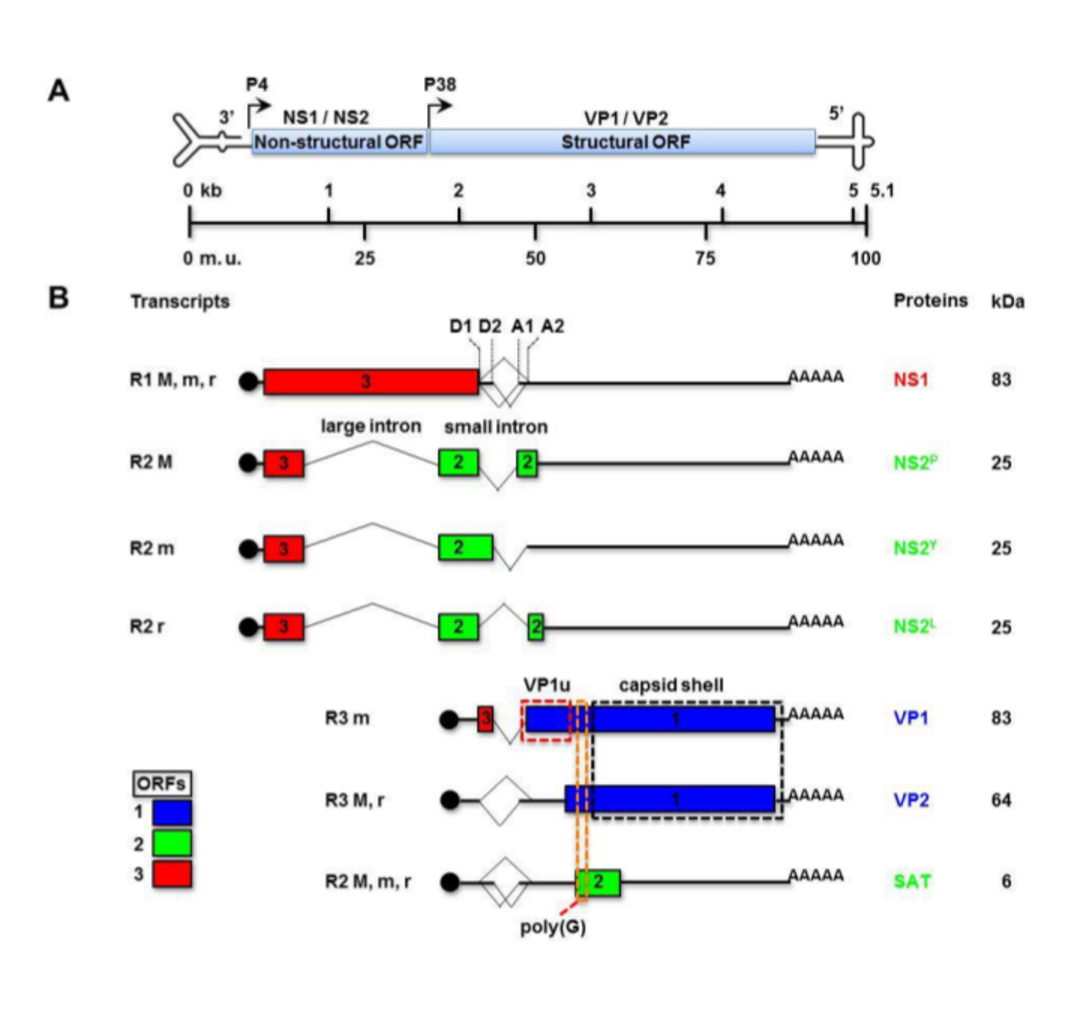
\includegraphics[scale=0.8]{Transcription}
  \caption[Transcription map of MVM]
   {Transcription map of MVM. \textbf{(A)} The single-stranded, negative-sense DNA genome of MVM is illustrated by a single line terminating in dissimilar hairpin telomeres. The two major ORFs are boxed in light blue and the proteins which they encode are indicated above. The two viral promoters, P4 and P38 are shown by rightward arrows. Below, arbitrary map units are diagrammed relative to the 5.1 kb genome. \textbf{(B)} The three major cytoplasmic transcript classes R1, R2, and R3 are displayed. A black sphere indicates the capped 5’ ends and (AAAAA) denotes their polyadenylated tails near the far right-hand end of the genome. ORFs encoding the viral proteins, named on the right, are displayed in different coloring according to their reading phase. Their spliced-out large or small introns are indicated by thin-lined carets. The small intron is excised from each transcript class by the alternative use of three different splicing patterns, denoted M (major), m (minor), and r (rare). Splice donor and acceptor sites for splicing of the small intron are denoted D1, D2 and A1, A2, respectively. On the one hand, alternative splicing of the small intron generates the R3 transcripts encoding VP1 and VP2, the two structural capsid proteins, and the R2 transcripts encoding three C-terminally distinct isoforms of NS2, referred to as NS2\textsuperscript{P}, NS2\textsuperscript{Y}, and NS2\textsuperscript{L}. On the other hand, excision of the large intron is critical in determining the steady state levels of NS1 and NS2 transcripts. The N-terminal protein sequence boxed in red represents VP1u which harbors the PLA\textsubscript{2} motif that is involved in entry functions. Sequences boxed in black, comprising the C-terminal region common to all VP polypeptides, assemble to form the capsid shell. Poly(G), boxed in orange, identifies a short glycine-rich region present in all VPs that can be modeled into X-ray density occupying the fivefold pores in virions. This figure was adapted from \cite{small}}
\label{Transcription}
\end{figure}       



\nomenclature{pre-mRNA}{messenger RNA precursor}
\nomenclature{mRNA}{messenger RNA}
\nomenclature{m.~u.}{Map units}
\nomenclature{ABP}{AMDV-binding protein}
\nomenclature{TfR}{Transferrin receptor}

\section{Assembly}
\label{Assembly}

The assembly of MVM capsids occurs in the nucleus and involves cytoplasmic trimerization of viral structural proteins and subsequent nuclear translocation of those trimers (see section~\ref{Struc Transloc}, p.~\pageref{Struc Transloc}) \cite{pmid16469332}. The formation of trimers results from extensive intertwinement of the VP polypeptides through extended surface loops which form tight, convoluted intratrimer interactions (see figure~\ref{Structure1}, p.~\pageref{Structure1}) \cite{pmid15299974, pmid21867712}. These trimers are incompetent for capsid assembly in the cytoplasm. In order to confer nuclear assembly, the trimeric precursors undergo a global conformational rearrangement on top of the 3-fold spike at the center of each trimer \cite{pmid16469332, pmid12552010, pmid17626084}. Nuclear association of trimeric assembly intermediates is mainly mediated by quasi-linear, hydrophobic interactions between trimeric subunits. Polar interactions only marginally contribute to capsid assembly and stability. Just a few conserved key residues which are invariably located at the intertrimer interfaces participate in the strongest interactions \cite{pmid14981262}.     

Currently, it remains uncertain whether auxiliary nuclear factors with chaperone activity are required for the final steps of parvovirus assembly and maturation. There is evidence that the formation of MVM capsids requires both nuclear factors and the major capsid protein VP2. Expressed capsid proteins that were incompetent for nuclear localization, as well as singly expressed nuclear transport competent VP1 proteins in the absence of VP2 proteins, were not able to assemble \cite{pmid12072505, pmid10438891, pmid10729155}. In the case of B19V it was demonstrated that VP1 deletion mutants formed morphologically normal capsids. However, only a limited extension of VP1 was tolerated. The longer the VP1 versions, the less efficient was assembly and assembled particles showed dysmorphic appearance \cite{pmid8207846}. Truncations beyond 30 amino acids at the N-terminus of VP2 prevented assembly because they affected the $\beta$A-strand of the conserved $\beta$-barrel motif which constitutes the core of the capsid shell (see figure~\ref{Structure1}, p.~\pageref{Structure1}) \cite{pmid7666560}.     


Nuclear assembly is decoupled to the S-phase of the host cell. Inhibition of DNA synthesis resulted in a reduction of mature virions. Nonetheless, empty capsids accumulated in the nucleus of infected cells \cite{pmid559779, assembly}. In contrast, the viral non-structural protein NS2 was reported to play a host-range specific role in MVM capsid assembly. On the one hand, MVM expressing truncated forms of NS2 was able to give rise to progeny virus in transformed human fibroblasts, albeit with reduced efficiency. On the other hand, they were unable to assemble in their restrictive murine host cells in spite of properly expressing NS1 and the structural proteins in early stages post-infection. The involvement of NS2 in virus assembly remains elusive but is likely to be indirect, since an appropriate cellular environment can complement the defect \cite{pmid9168889}.        


A profound understanding of the mechanisms of capsid assembly and disassembly shows great promise for the development of antiviral drugs. Virus propagation may be prevented by interference with capsid assembly or by promoting or inhibiting capsid disassembly \cite{pmid21762804, pmid21163649}. Further applications may be the use of self-assembling nanoparticles for biomedical and nanotechnological applications \cite{pmid16521330, pmid16690856}.     


  
\section{DNA Packaging}
\label{Packaging}

Generally, viruses use two alternative strategies to package their genomes into the capsids. On the one hand, viruses containing circular dsDNA genomes assemble their protein shell around the genome, driven by interactions between protein capsid subunits and nucleic acids \cite{pmid6101085, pmid6305987, pmid1323699}. Moreover, several ssDNA or ssRNA viruses, such as tobacco mosaic virus, F1, and M13 bacteriophage follow the same assembly pathway via association of structural proteins around the genome \cite{pmid11406604}. On the other hand, viruses with double-stranded linear genomes translocate their genetic material into pre-assembled empty capsids. This process is ATP-dependent and involves auxiliary non-structural packaging enzymes \cite{pmid2679356}. The presence of a large excess of empty capsids in parvovirus stocks and the fact that single expression of their structural proteins is sufficient for capsid formation \cite{pmid1331503} implies that the viral DNA is not required for capsid assembly. Thus, parvoviruses use the latter mechanism for genome translocation into their pre-formed capsids which accumulate in the cell nucleus (see section~\ref{Assembly}, p.~\pageref{Assembly}). Significantly, the encapsidation process has been visualized by EM in an \textit{in vitro} assembly and packaging reaction of Lu\RM{3} parvovirus \cite{pmid6221078}.

In the case of MVM, partially or fully packaged capsids were demonstrated to interact with NS1. The non-structural protein was covalently attached to the 5' termini of unit-length ssDNA genomes. These structures may represent intermediates of the packaging process which could be supported by NS1, particularly its 3' to 5' helicase activity (see section XY..) \cite{pmid2527311}. Similar observations were reported for AAV2 capsids which were shown to interact with \textit{rep} proteins \cite{pmid8553536, pmid8995658}. DNase protection studies in AAV \cite{pmid11406604} and DNA to capsid binding experiments of autonomous parvoviruses \cite{pmid2145445, pmid8350419} suggest a 3’ to 5’ packaging direction for parvoviruses. According to the directionality of the encapsidation process, the 3’ to 5’ processivity of the virus-encoded helicase, rather than the strand displacement RHR synthesis, seem to drive the translocation of the genome into pre-formed capsids \cite{pmid11406604}. 

Initiation of the encapsidation process involves viral \textit{cis}-acting elements. The ITRs of AAV contain a packaging signal which is both required and sufficient for genome encapsidation \cite{pmid2547998}. Currently, a direct, specific interaction of AAV ITRs with capsids has not yet been demonstrated \cite{pmid8627687, pmid9060669}. In contrast, specific binding of the 3' terminal repeat of MVM to VP1 \cite{pmid1870193} and to particles composed only of VP2 \cite{pmid8350419} has been reported. However, binding to VP1 is not essential since VP1 is dispensable for MVM assembly and packaging \cite{pmid8416366}.      

Cross-packaging of Lu\RM{3}-derived vector genomes into capsids of MVM reinforced the observation that strand selection for packaging occurs due to varying efficiency of excision from replicated genomes of one strand polarity \textit{versus} the other rather than differences in packaging preference \cite{pmid15866075}. This phenomenon is further elucidated in section~\ref{Resolution}, p.~\pageref{Resolution}.    

\section{Nuclear Export}

Besides having the possibility to passively egress the host cell by NS1-induced cellular lysis, the latest data of several research groups suggest an active, pre-lytic egress for MVM \cite{pmid24068925, pmid18704167, pmid15367635}. In order to actively egress the host cell, progeny particles of karyophilic viruses need to cross considerable cellular barriers. Apart from the plasma membrane, the nuclear envelope constitutes a second barrier to MVM. Although the mechanism for nuclear export and subsequent release of MVM virions remains elusive, several important viral and cellular effectors involved in PV egress have been identified and characterized. 

MVM is exported from the host’s nucleus by a Crm1 dependent mechanism. Stable interaction of NS2 with Crm1 was successfully demonstrated \cite{pmid10438867, pmid10527855}. Classical nuclear export signals (NES) exhibit low affinity for Crm1 to prevent from the formation of the Crm1/cargo complex in the cytoplasm where RanGTP is absent \cite{pmid10449743}. Surprisingly, the NES of NS2 belongs to the supraphysiological NES which tightly bind to Crm1 regardless of the presence of RanGTP. Therefore, NS2 competitively inhibits Crm1 function by sequestering endogenous nuclear export receptors \cite{pmid18385513}. MVM mutant genomic clones generating NS2 proteins harbouring either regular NES, or substitutions which abrogated Crm1 interaction were shown to be compromised in viral nuclear export and productive infection. 

As expected, NS2-Crm1-mutants showed nuclear accumulation of export deficient NS2 in transfected cells. Surprisingly, the nuclear retention of mutant NS2 proteins came along with a substantial accumulation of progeny virions in the nucleus of infected cells, suggesting a NS2-dependent export of progeny virions. Additionally, an indirect involvement of NS2 in viral egress was demonstrated using the closely related H1-PV. An in-frame deletion of 38 amino acids within the common coding sequence of NS1 and NS2 was demonstrated to beneficially influence virus infectivity \textit{in vitro}, indicated by a lower particle-to-infectivity (P/I) ratio and a larger plaque phenotype. The increase in infectivity, which resulted from an accelerated egress of the mutant progeny virions, positively affected tumor growth suppression \textit{in vivo} \cite{pmid22553326}. However, approaches to demonstrate a direct interaction between NS2 and the viral capsid and/or individual structural proteins \textit{in vitro} have not yet been successful.  


The differences in nuclear export observed during productive MVM infection in either permissive human cells or restrictive murine cells may result from the cell-type-specific use of alternative strategies for nuclear export. It became apparent when the different cell types were treated with the anti-fungal antibiotic leptomycin B (LMB), a drug which inhibits Crm1-dependent nuclear export \cite{pmid9683540}. LMB treatment of susceptible murine cells resulted in a significant but not complete inhibition of nuclear export of MVM progeny virions. In contrast, even high doses of LMB did not inhibit nuclear export of MVM in transformed human cells, indicating that Crm1 is not essentially involved in the nuclear export of MVM in these cells \cite{pmid15367635}. The observed differences may result from a cell-type dependent phosphorylation status of MVM. Generally, MVM capsids derived from permissive human cells displayed prominent phosphorylation compared to the decent phosphorylation status of capsids isolated from restrictive murine fibroblasts \cite{pmid11069983}. Significantly, the three distal serine residues at position 2, 6, and 10 of the unordered N-VP2 terminus showed high phosphorylation levels in permissive cells. Site-directed mutagenesis verified an important role of these phosphorylations in the Crm1-independent nuclear export of MVM in permissive human cells. When the N-terminal phosphorylations were diminished, progeny virions were predominantly retained in the nucleus and the corresponding mutants displayed a small plaque phenotype, indicating the importance of those phosphorylations in viral spread \cite{pmid15367635}. 

\nomenclature{LMB}{Leptomycin B}  

\section{Egress}

MVM transport from the nucleus to the cell periphery is associated with the degradation of actin fibers and the formation of “actin-patches”. These alterations to the filamentous network were attributed to a virus-induced imbalance between the actin polymerization factor neural Wiskott-Aldrich syndrome protein (N-WASP) and gelsolin, a member of the actin-severing protein family \cite{pmid15582663}. Indeed, the MVM titer in the culture supernatant following MVM infection drastically declined when gelsolin function was diminished. During MVM infection, gelsolin activity is regulated by the CK\RM{2}$\alpha$/NS1 complex which was demonstrated to be capable of phosphorylating gelsolin. Consequentially, inhibition of CK\RM{2}$\alpha$ correlated with prolonged persistence of actin fibers and delayed formation of the characteristic “actin patches” \cite{pmid18704167, pmid16641266}. Several lines of evidence coincide with an active, vesicle-associated, gelsolin-dependent export of MVM. Progeny virions were shown to co-localize with exocytic, endosomal, and lysosomal markers in immunofluorescent experiments \cite{pmid18704167, pmid17287256}. Cell fractionation experiments confirmed this hypothesis by demonstrating a co-migration of viral particles with cytosolic vesicles rather than free, vesicle-independent localization in the soluble cytosolic fraction. Moreover, dynamin was found to accumulate in the perinuclear region where it co-localized with de novo synthesized MVM capsids. A cooperative cross-talk between actin- and microtubule dependent transport \cite{pmid15040446, pmid12383793, pmid17998399} might be involved in MVM transport from the nucleus to the cell periphery, resulting in the destruction of actin filaments and the stabilization of microtubules \cite{pmid18704167}.  
The secretion pathway represents the proposed route for active egress of MVM. It is supposed that progeny virions become engulfed by COPII-vesicle formation in the perinuclear endoplasmic reticulum (ER). In order to verify this hypothesis, cells lacking functional effectors of the secretory pathway were productively infected.  Accordingly, a dramatic retention of virions in the perinuclear area was observed, accompanied by inhibited virion release into the medium. Contrarily, no significant co-localization between MVM progeny virions and representative markers of the recycling pathway or the Trans Golgi Network (TGN) were evident \cite{pmid24068925}. In addition, members of the ezrin, radixin, and moesin (ERM) protein family, such as radixin and moesin, were shown to play a role in virus maturation and spreading capacity, as judged by their impact on MVM plaque morphology \cite{pmid19321616}. Indeed, dominant negative radixin or moesin mutants failed in wrapping progeny virions into transport vesicles, resulting in a marked reduction of egressed virions in the culture supernatant. As a consequence, corresponding markers for alternative export routes, e.g. direct transport from the TGN to the PM or through recycling endosomes, exhibited increased co-localization with progeny virions. Finally, active egress promotes cellular lysis as demonstrated by the prolonged viability of cells in which vesicular transport was either inhibited or by-passing the Golgi apparatus. Besides, the involvement of progeny particles in cytolysis was demonstrated by the prolonged survival of murine cells transduced with a viral vector deficient for the production of progeny virion particles \cite{pmid24068925}.  




\begin{figure}
\centering
  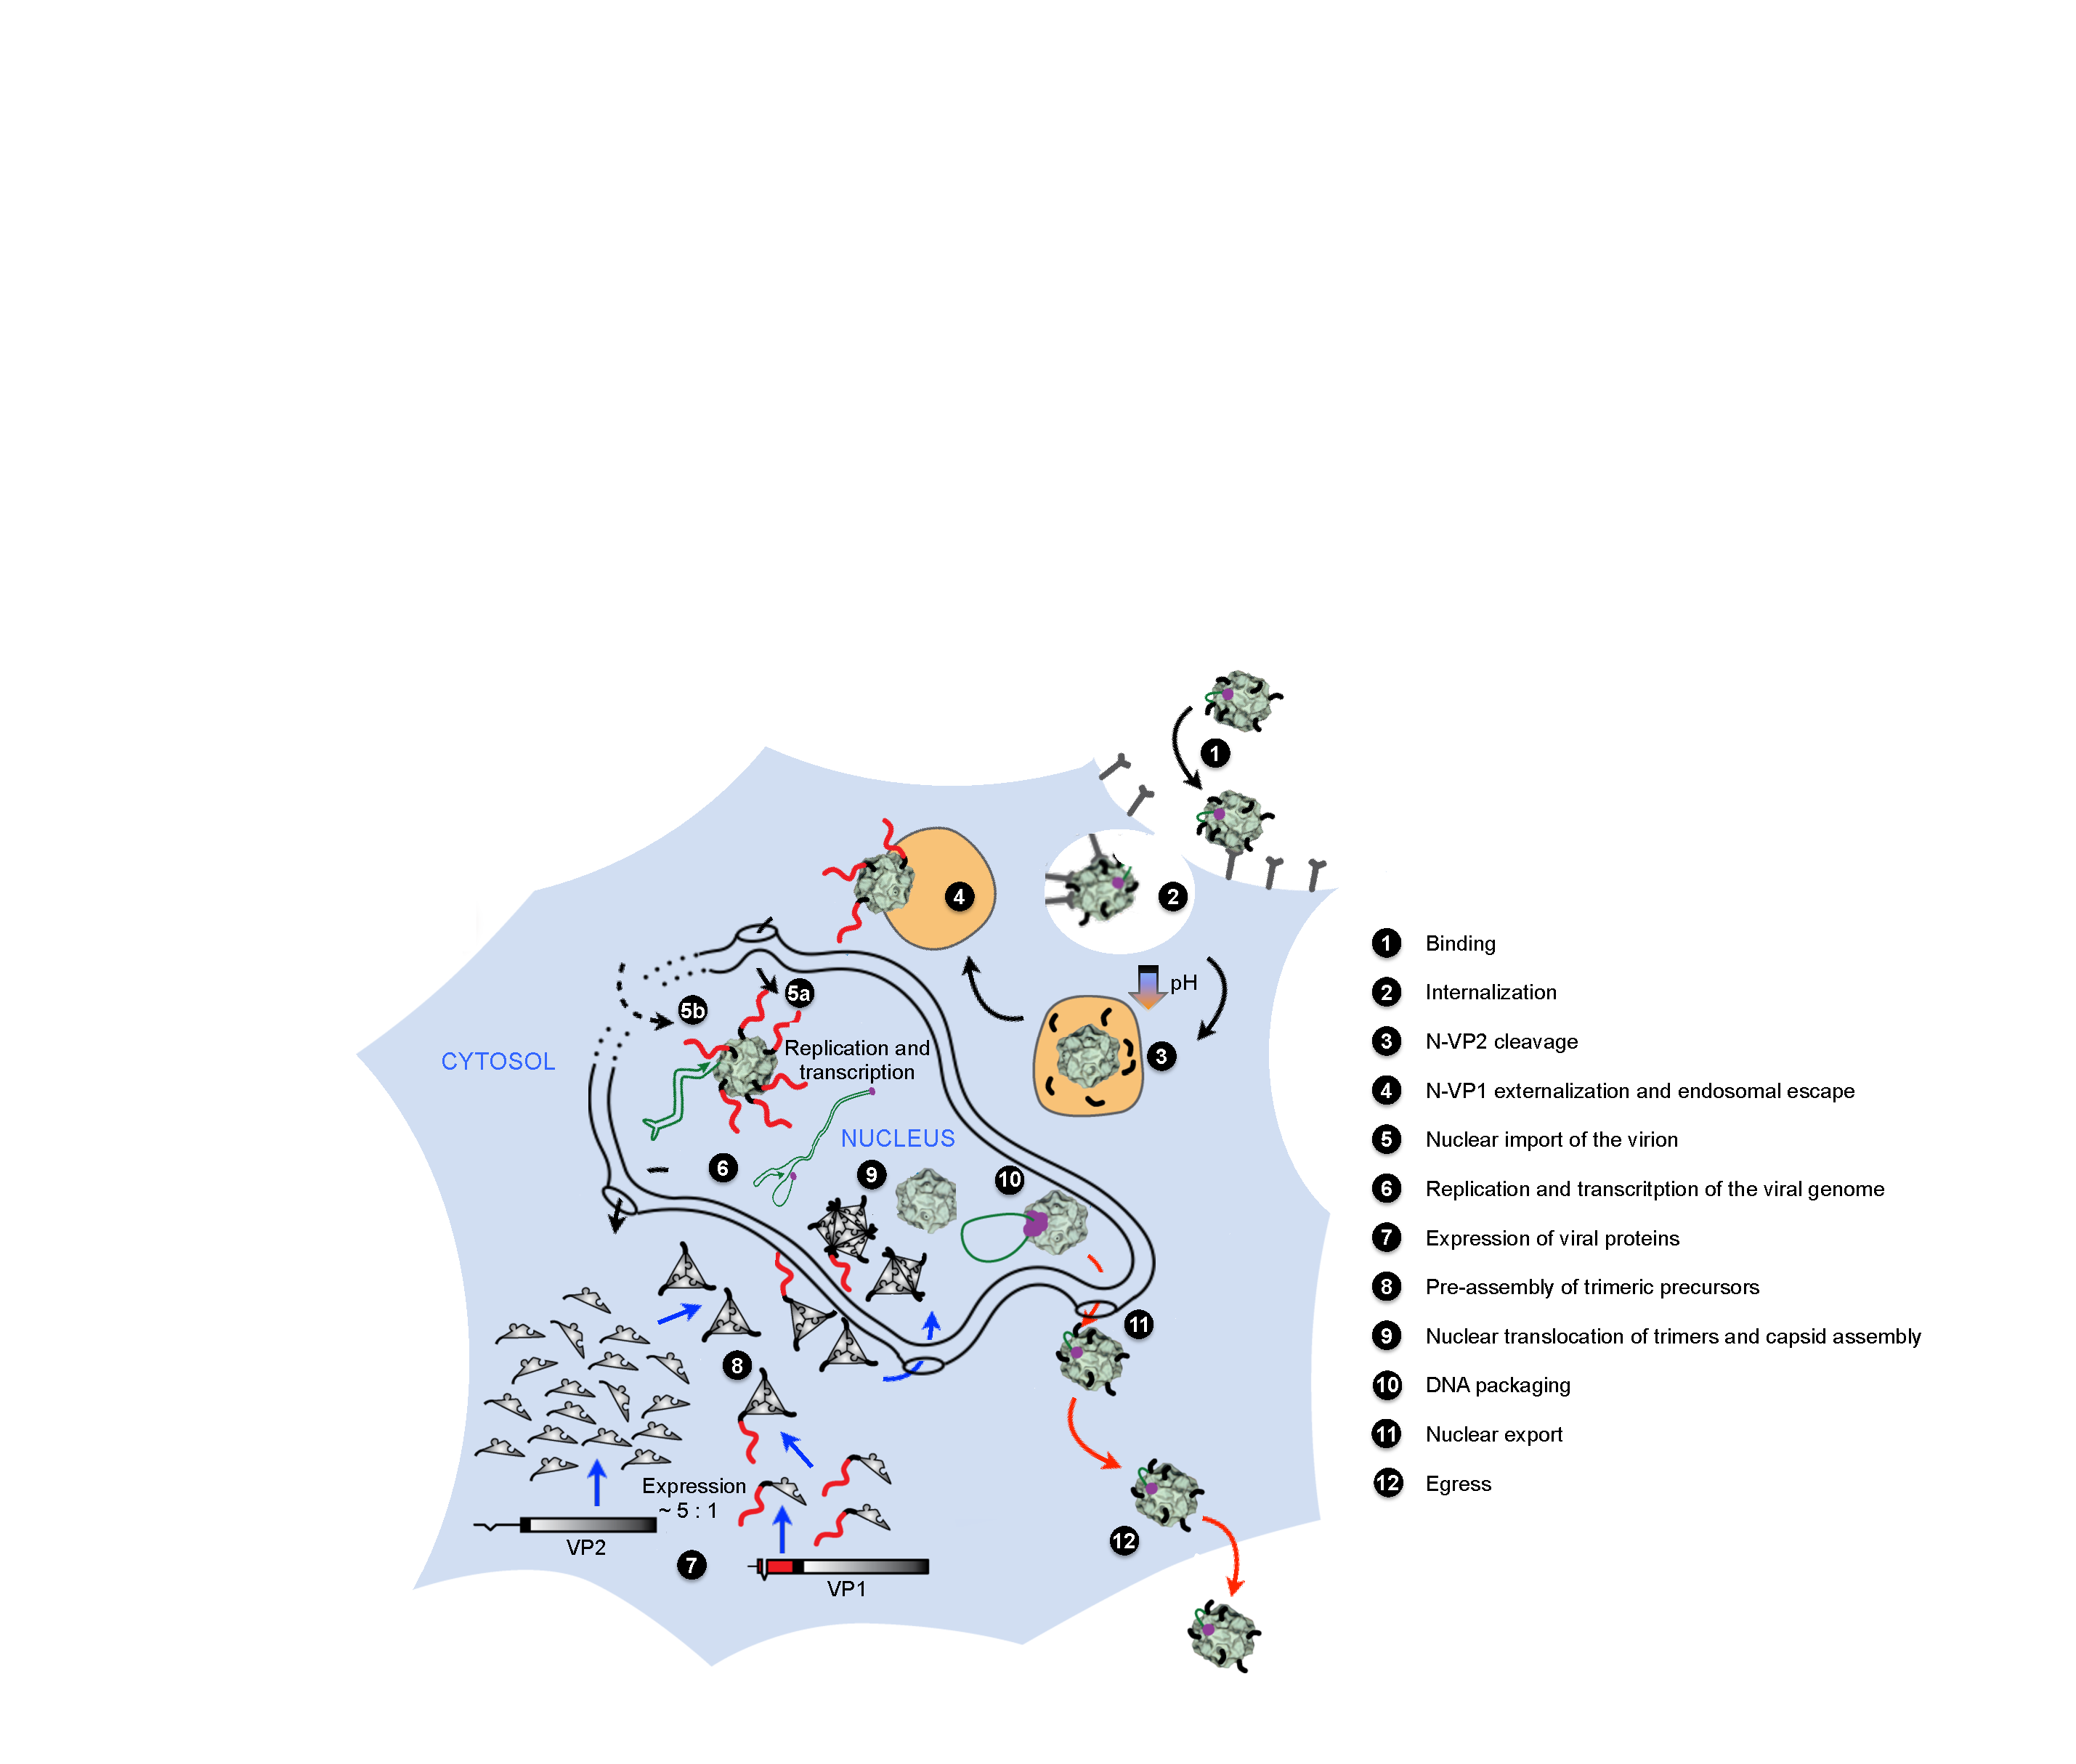
\includegraphics[scale=0.4]{Cycle}
  \caption[Life cycle of MVM]
   {Simplistic view of the life cycle of MVM. Cell entry (black arrows), protein expression and progeny assembly (blue arrows), and DNA packaging, nuclear export and egress (red arrows) are illustrated schematically. The unknown cell surface receptors are indicated as extended Y shapes and acidic late endocytic vesicles are colored in orange. Colored lines associated with virus particles represent the flexible N-VP2 termini (black), the VP1u region (red) and the viral genomic DNA (green). The number of externalized N-VP1 termini is not known and might vary between one and ten. Currently, nuclear targeting (see step 5) of the virion is controversial and remains elusive. Due to its small size, MVM could physically traverse the NPC fully intact (see 5a). Alternatively, MVM was suggested to enter the nucleus in an NPC-independent manner by partial disruption of the nuclear envelope (5b). Horizontal bars represent primary VP gene transcripts and jigsaw triangles indicate the folded core containing the jellyroll motif common to all VP polypeptides. The multifunctional non-structural NS1 protein, which assists DNA replication and packaging, is represented as purple sphere. This schematic representation is not drawn to scale and was adapted from reference \cite{small}.  
} 
\label{Cycle}
\end{figure}






    

\nomenclature{TGN}{Trans Golgi network}
\nomenclature{N-WASP}{Neural Wiskott-Aldrich syndrome protein}
\nomenclature{ER}{Endoplasmic reticulum}
\nomenclature{ERM}{Ezrin, radixin, and moesin}

